% Editable native annotations around unchanged verified IDE photographs.
\par
\begin{figure}[htbp]
  \centering
  \newsavebox{\MARSqoiencodedregistersBox}
  \sbox{\MARSqoiencodedregistersBox}{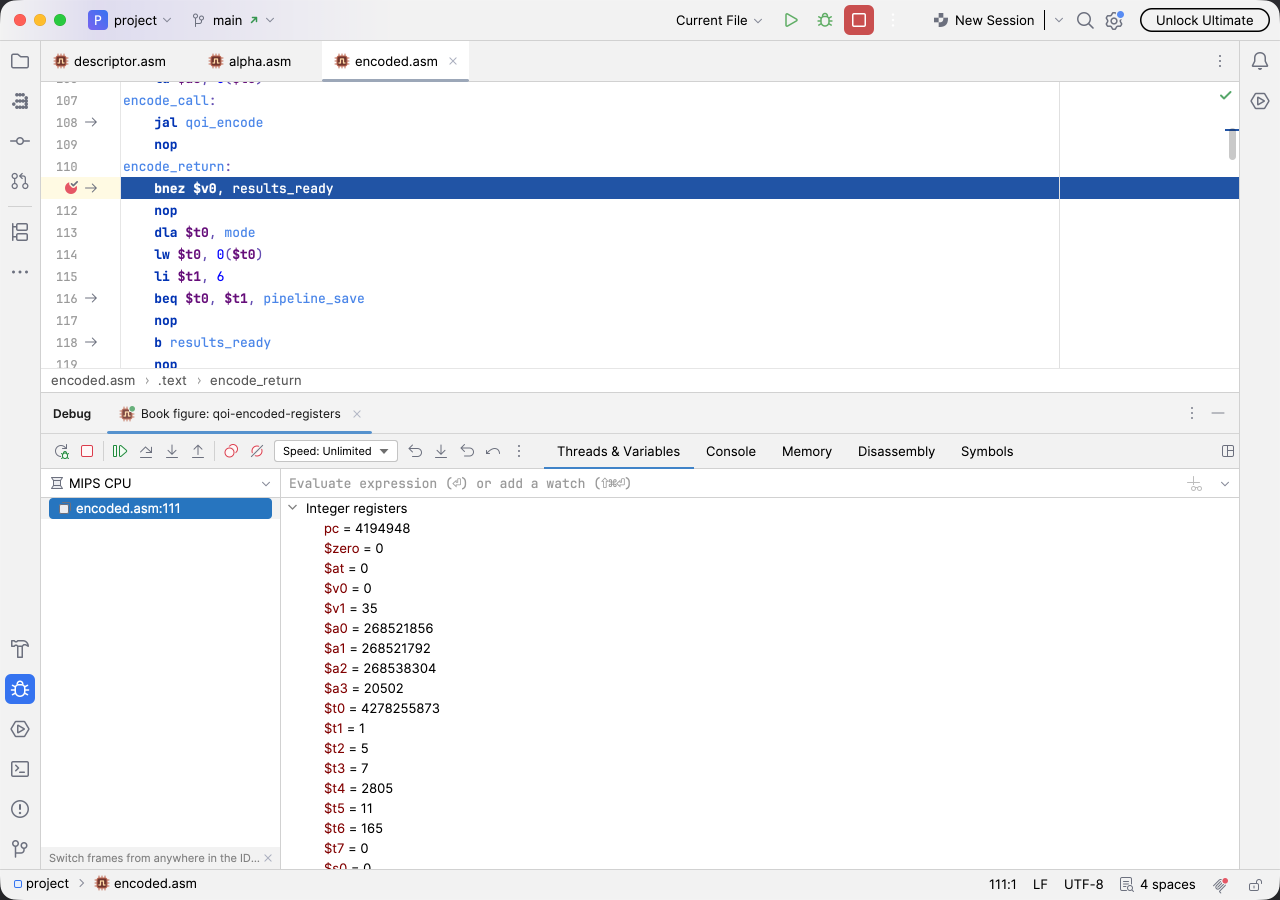
\includegraphics[artifact]{packages/030-qoi/captures/f03/registers.png}}
  \newsavebox{\MARSqoiencodedoutputBox}
  \sbox{\MARSqoiencodedoutputBox}{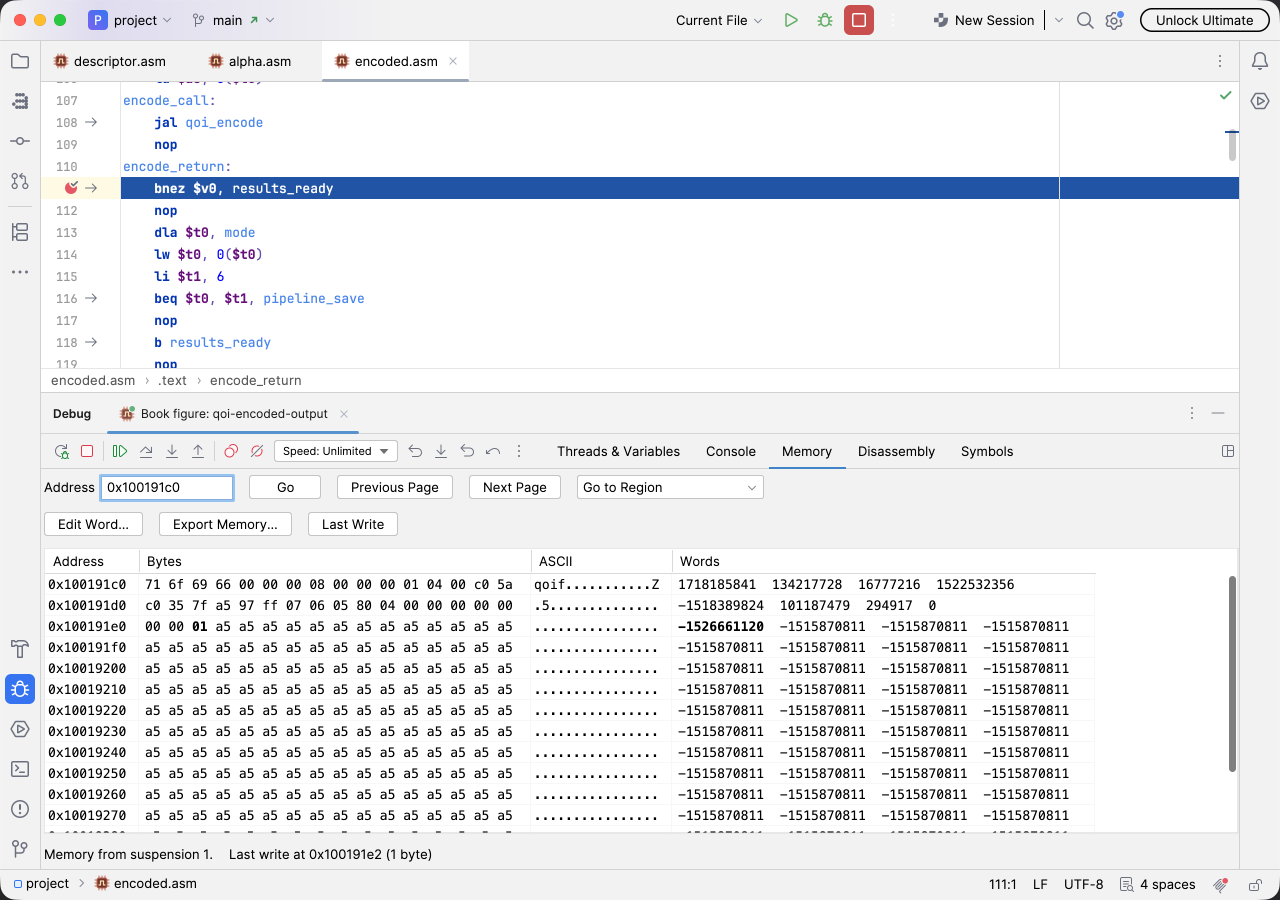
\includegraphics[artifact]{packages/030-qoi/captures/f03/output.png}}
  \newsavebox{\MARSqoiencodedframebufferBox}
  \sbox{\MARSqoiencodedframebufferBox}{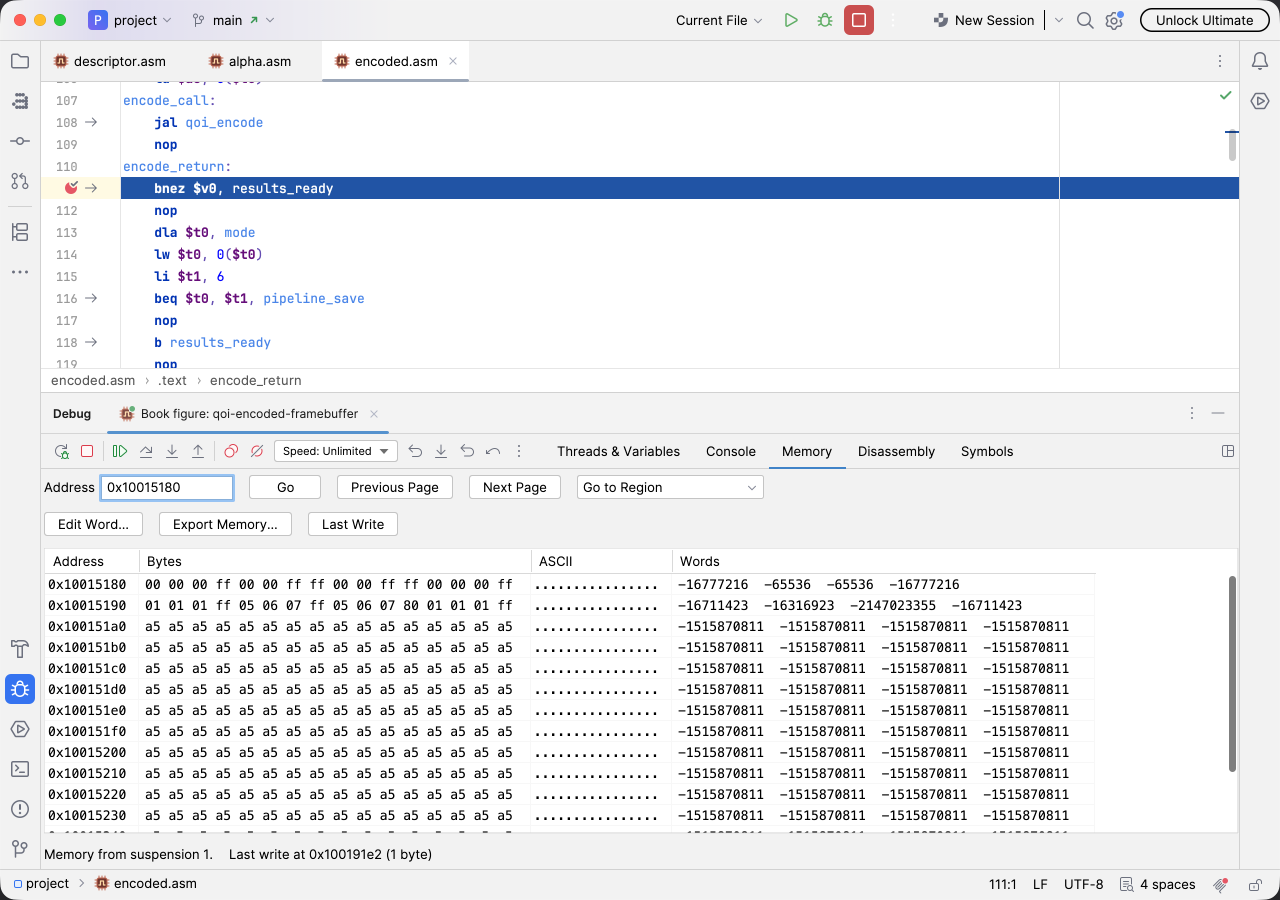
\includegraphics[artifact]{packages/030-qoi/captures/f03/framebuffer.png}}
  \newsavebox{\MARSqoiencodedmetadataBox}
  \sbox{\MARSqoiencodedmetadataBox}{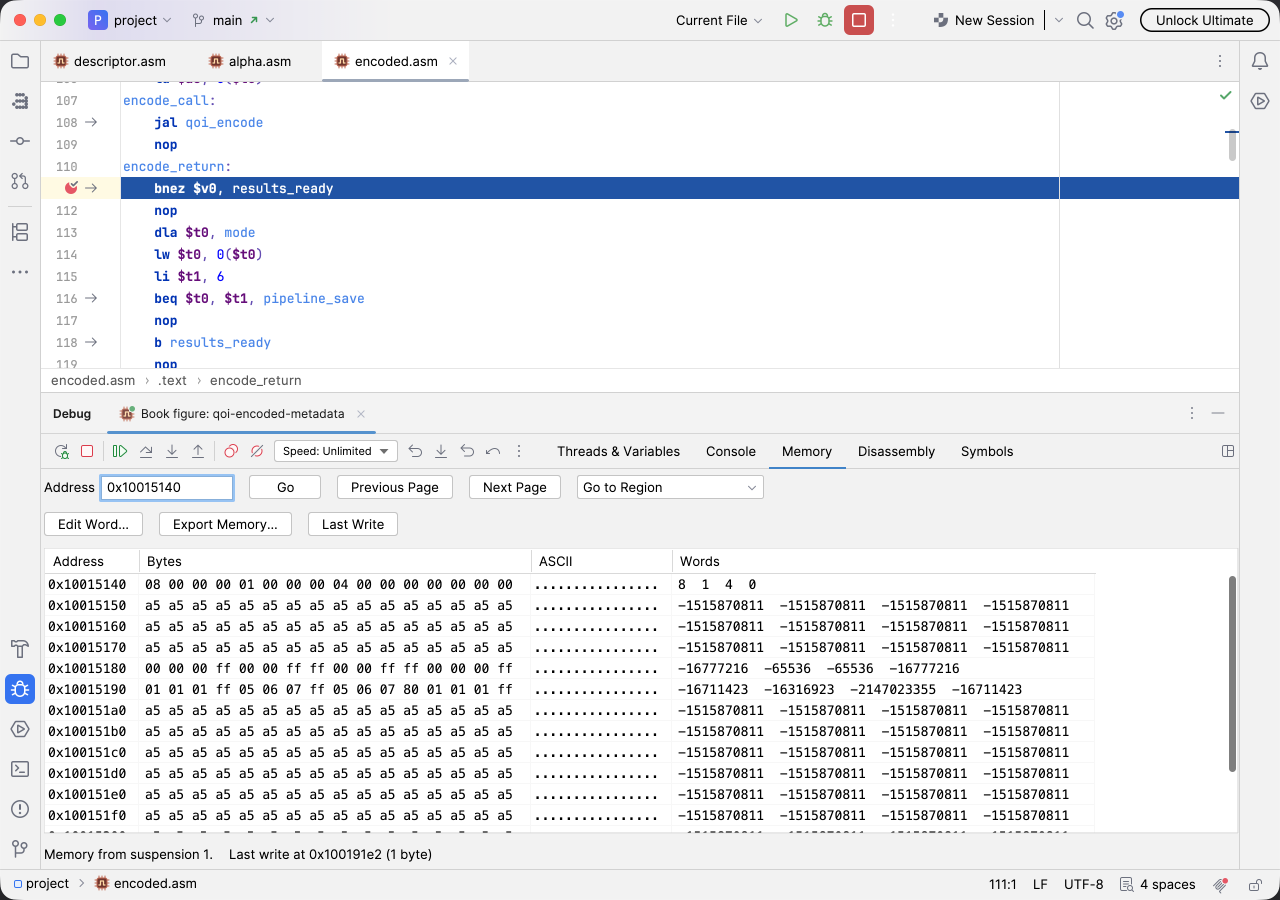
\includegraphics[artifact]{packages/030-qoi/captures/f03/metadata.png}}
  \edef\MARSqoiencodedsourceLeft{\the\dimexpr0.036718750\wd\MARSqoiencodedregistersBox\relax}
  \edef\MARSqoiencodedsourceBottom{\the\dimexpr0.774444444\ht\MARSqoiencodedregistersBox\relax}
  \edef\MARSqoiencodedsourceRight{\the\dimexpr0.713281250\wd\MARSqoiencodedregistersBox\relax}
  \edef\MARSqoiencodedsourceTop{\the\dimexpr0.170000000\ht\MARSqoiencodedregistersBox\relax}
  \edef\MARSqoiencodedreturnsLeft{\the\dimexpr0.246093750\wd\MARSqoiencodedregistersBox\relax}
  \edef\MARSqoiencodedreturnsBottom{\the\dimexpr0.312222222\ht\MARSqoiencodedregistersBox\relax}
  \edef\MARSqoiencodedreturnsRight{\the\dimexpr0.553906250\wd\MARSqoiencodedregistersBox\relax}
  \edef\MARSqoiencodedreturnsTop{\the\dimexpr0.640000000\ht\MARSqoiencodedregistersBox\relax}
  \edef\MARSqoiencodedoutputLeft{\the\dimexpr0.034375000\wd\MARSqoiencodedoutputBox\relax}
  \edef\MARSqoiencodedoutputBottom{\the\dimexpr0.287777778\ht\MARSqoiencodedoutputBox\relax}
  \edef\MARSqoiencodedoutputRight{\the\dimexpr0.584375000\wd\MARSqoiencodedoutputBox\relax}
  \edef\MARSqoiencodedoutputTop{\the\dimexpr0.608888889\ht\MARSqoiencodedoutputBox\relax}
  \edef\MARSqoiencodedinputLeft{\the\dimexpr0.034375000\wd\MARSqoiencodedframebufferBox\relax}
  \edef\MARSqoiencodedinputBottom{\the\dimexpr0.311111111\ht\MARSqoiencodedframebufferBox\relax}
  \edef\MARSqoiencodedinputRight{\the\dimexpr0.584375000\wd\MARSqoiencodedframebufferBox\relax}
  \edef\MARSqoiencodedinputTop{\the\dimexpr0.608888889\ht\MARSqoiencodedframebufferBox\relax}
  \edef\MARSqoiencodedmetadataLeft{\the\dimexpr0.034375000\wd\MARSqoiencodedmetadataBox\relax}
  \edef\MARSqoiencodedmetadataBottom{\the\dimexpr0.334444444\ht\MARSqoiencodedmetadataBox\relax}
  \edef\MARSqoiencodedmetadataRight{\the\dimexpr0.584375000\wd\MARSqoiencodedmetadataBox\relax}
  \edef\MARSqoiencodedmetadataTop{\the\dimexpr0.608888889\ht\MARSqoiencodedmetadataBox\relax}
  \begin{tikzpicture}[alt={Five details at encode_return show status zero and thirty-five bytes, the exact encoded QOI stream with a one-byte 5a difference chunk, original eight RGBA words, and metadata fields eight one four zero.}]
    \node[anchor=north west,inner sep=0,font=\small\bfseries] (source-title) at (6mm,0) {Caller instruction after encoding};
    \node[anchor=north west,inner sep=0] (source) at ([yshift=-1mm]source-title.south west) {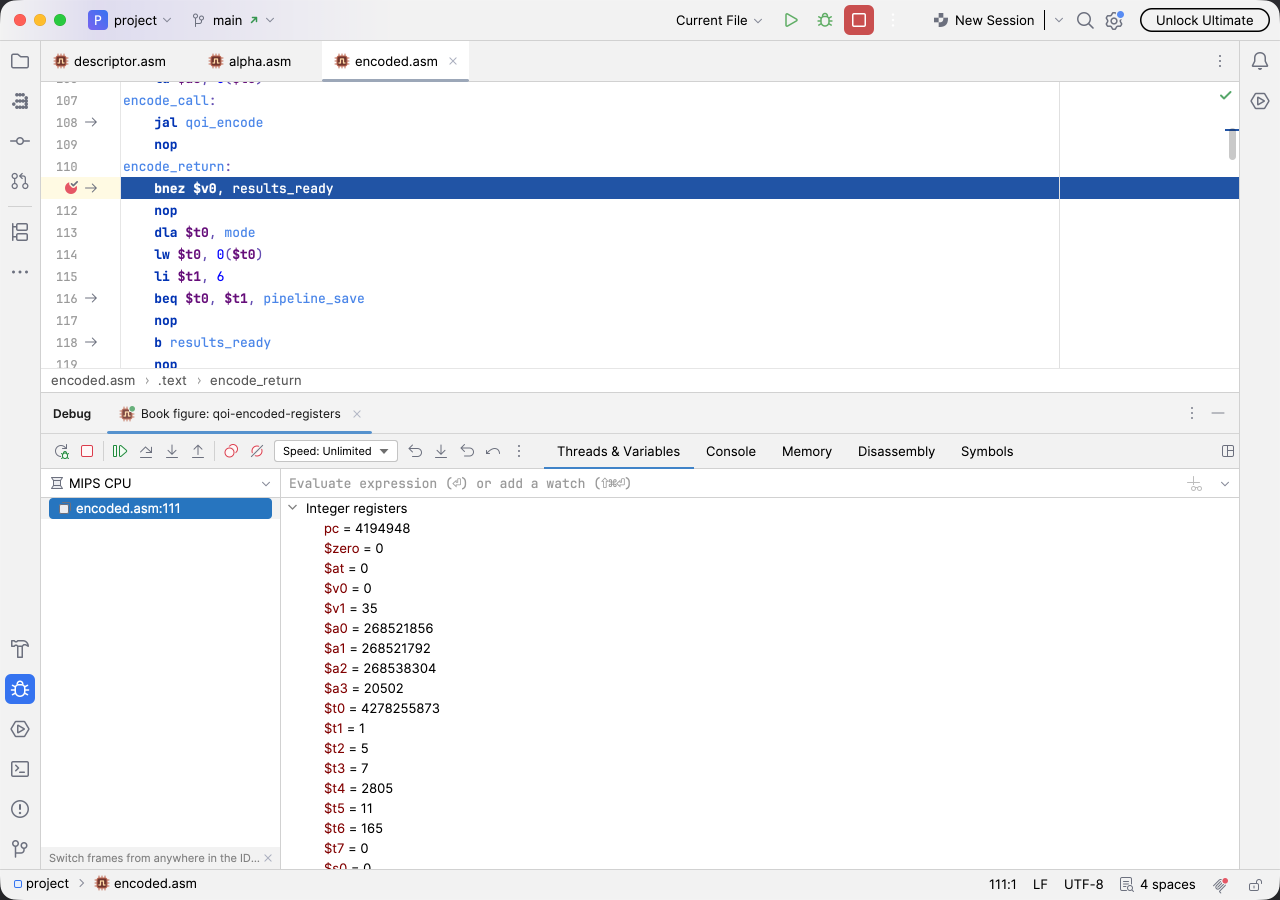
\includegraphics[width=0.54\linewidth,artifact,trim={\MARSqoiencodedsourceLeft{} \MARSqoiencodedsourceBottom{} \MARSqoiencodedsourceRight{} \MARSqoiencodedsourceTop{}},clip]{packages/030-qoi/captures/f03/registers.png}};
    \begin{scope}[shift={(source.south west)},x={($(source.south east)-(source.south west)$)},y={($(source.north west)-(source.south west)$)}]
      \draw[black,line width=0.7pt] (0.237500000,0.080000000) rectangle (0.893750000,0.520000000);
      \node[draw=black,fill=white,circle,inner sep=1.5pt,font=\footnotesize] at ($(0.237500000,0.520000000)+(-3mm,0)$) {1};
    \end{scope}
    \node[anchor=north west,inner sep=0,font=\small\bfseries] (returns-title) at ([yshift=-1mm]source.south west) {Success status and complete byte length};
    \node[anchor=north west,inner sep=0] (returns) at ([yshift=-1mm]returns-title.south west) {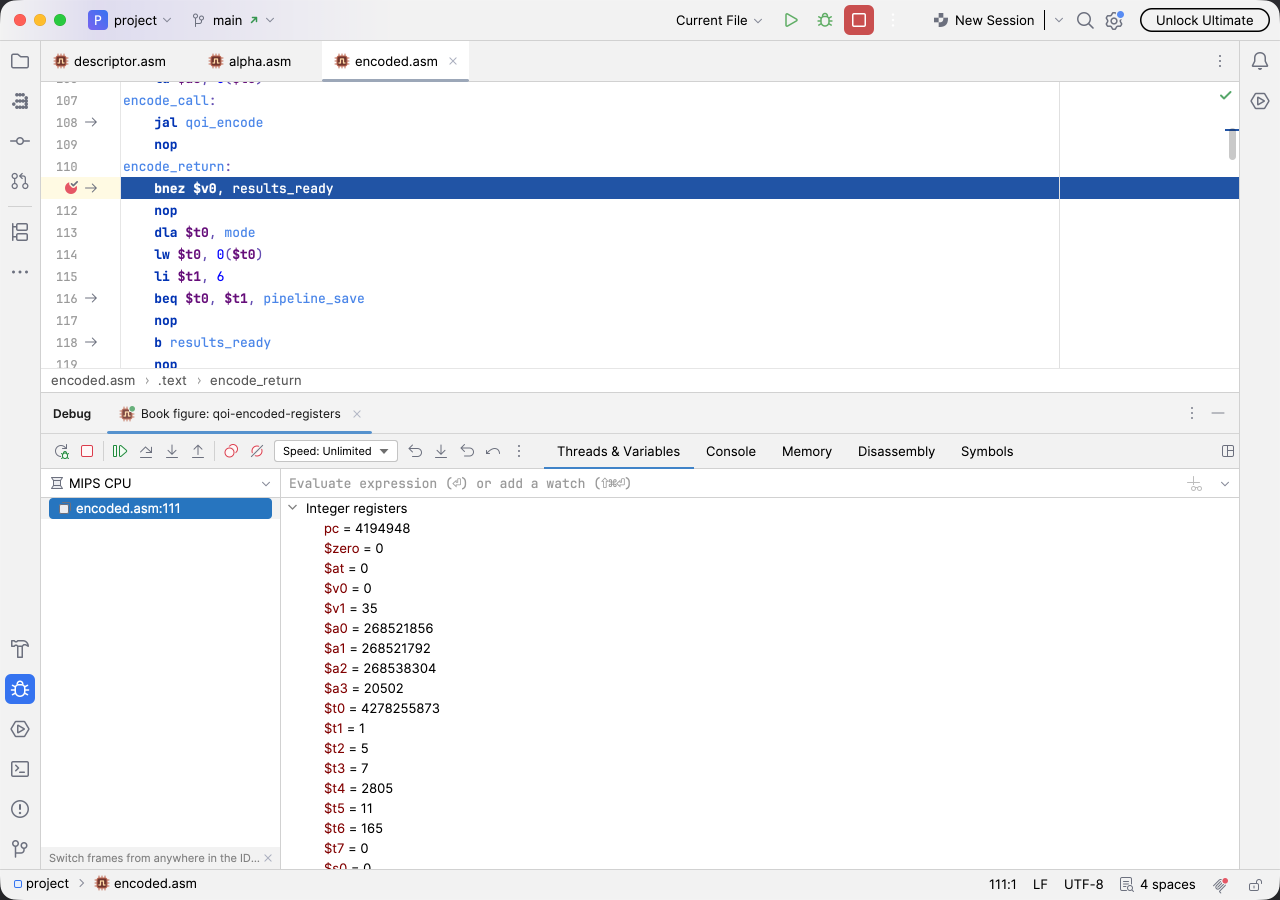
\includegraphics[width=0.48\linewidth,artifact,trim={\MARSqoiencodedreturnsLeft{} \MARSqoiencodedreturnsBottom{} \MARSqoiencodedreturnsRight{} \MARSqoiencodedreturnsTop{}},clip]{packages/030-qoi/captures/f03/registers.png}};
    \begin{scope}[shift={(returns.south west)},x={($(returns.south east)-(returns.south west)$)},y={($(returns.north west)-(returns.south west)$)}]
      \draw[black,line width=0.7pt] (0.023437500,0.023255814) rectangle (0.250000000,0.953488372);
      \node[draw=black,fill=white,circle,inner sep=1.5pt,font=\footnotesize] at ($(0.023437500,0.953488372)+(-3mm,0)$) {2};
    \end{scope}
    \node[anchor=north west,inner sep=0,font=\small\bfseries] (output-title) at ([yshift=-1mm]returns.south west) {Thirty-five-byte lossless QOI stream};
    \node[anchor=north west,inner sep=0] (output) at ([yshift=-1mm]output-title.south west) {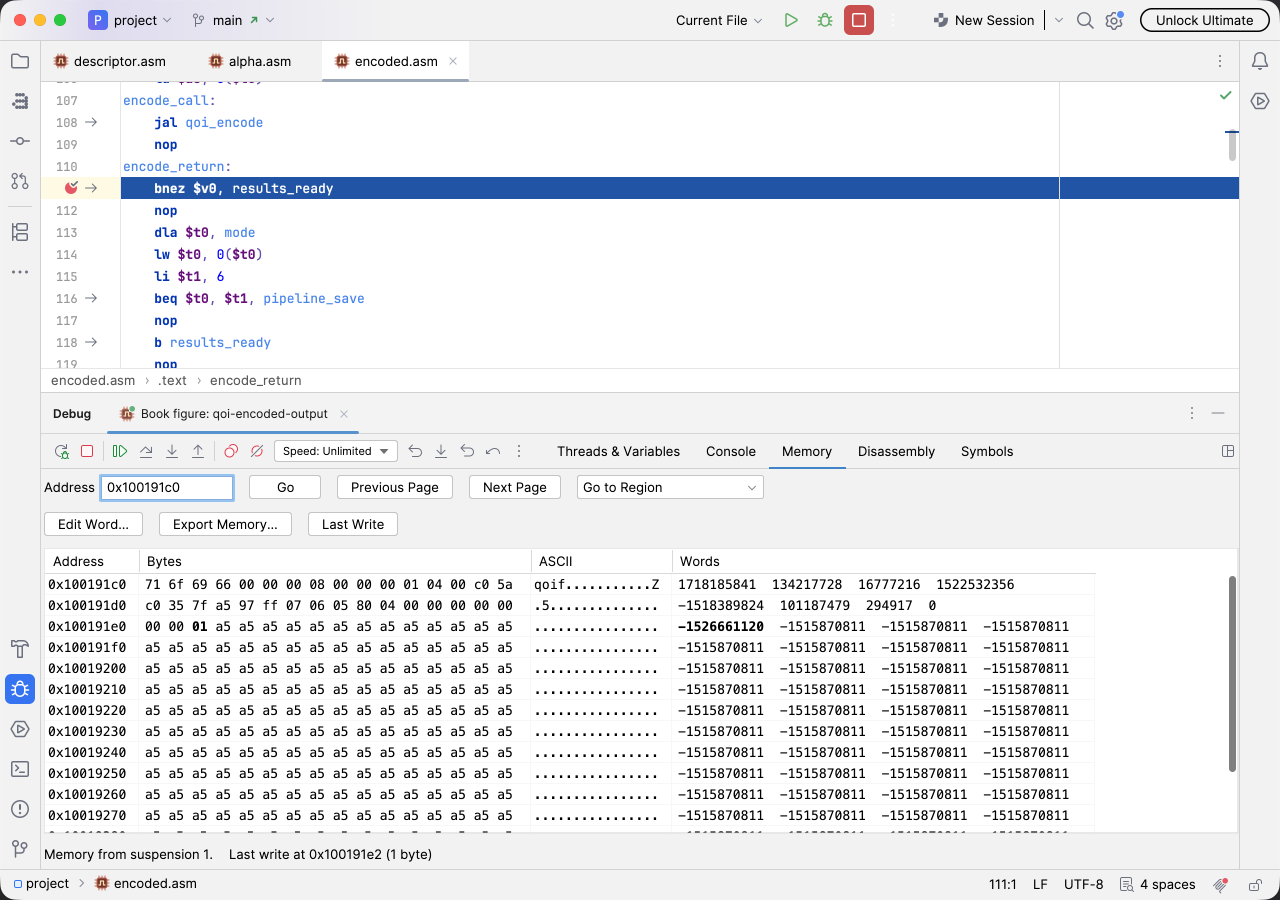
\includegraphics[width=0.84\linewidth,artifact,trim={\MARSqoiencodedoutputLeft{} \MARSqoiencodedoutputBottom{} \MARSqoiencodedoutputRight{} \MARSqoiencodedoutputTop{}},clip]{packages/030-qoi/captures/f03/output.png}};
    \begin{scope}[shift={(output.south west)},x={($(output.south east)-(output.south west)$)},y={($(output.north west)-(output.south west)$)}]
      \draw[black,line width=0.7pt] (0.194672131,0.043010753) rectangle (0.997950820,0.720430108);
      \node[draw=black,fill=white,circle,inner sep=1.5pt,font=\footnotesize] at ($(0,0.720430108)+(-3mm,0)$) {3};
    \end{scope}
    \node[anchor=north west,inner sep=0,font=\small\bfseries] (input-title) at ([yshift=-1mm]output.south west) {Unchanged original pixel words};
    \node[anchor=north west,inner sep=0] (input) at ([yshift=-1mm]input-title.south west) {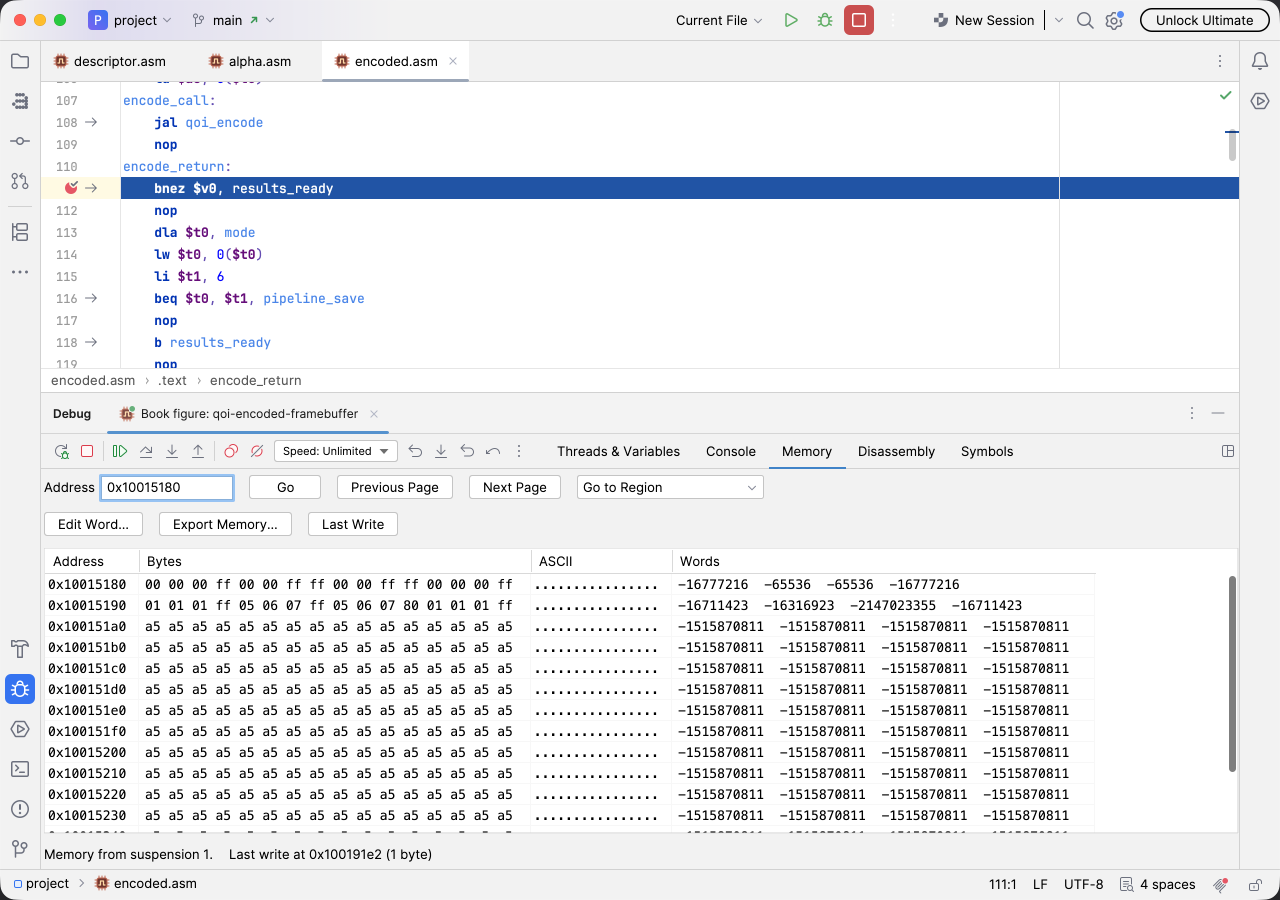
\includegraphics[width=0.84\linewidth,artifact,trim={\MARSqoiencodedinputLeft{} \MARSqoiencodedinputBottom{} \MARSqoiencodedinputRight{} \MARSqoiencodedinputTop{}},clip]{packages/030-qoi/captures/f03/framebuffer.png}};
    \begin{scope}[shift={(input.south west)},x={($(input.south east)-(input.south west)$)},y={($(input.north west)-(input.south west)$)}]
      \draw[black,line width=0.7pt] (0.194672131,0.055555556) rectangle (0.997950820,0.638888889);
      \node[draw=black,fill=white,circle,inner sep=1.5pt,font=\footnotesize] at ($(0,0.638888889)+(-3mm,0)$) {4};
    \end{scope}
    \node[anchor=north west,inner sep=0,font=\small\bfseries] (metadata-title) at ([yshift=-1mm]input.south west) {Unchanged dimensions and descriptive flags};
    \node[anchor=north west,inner sep=0] (metadata) at ([yshift=-1mm]metadata-title.south west) {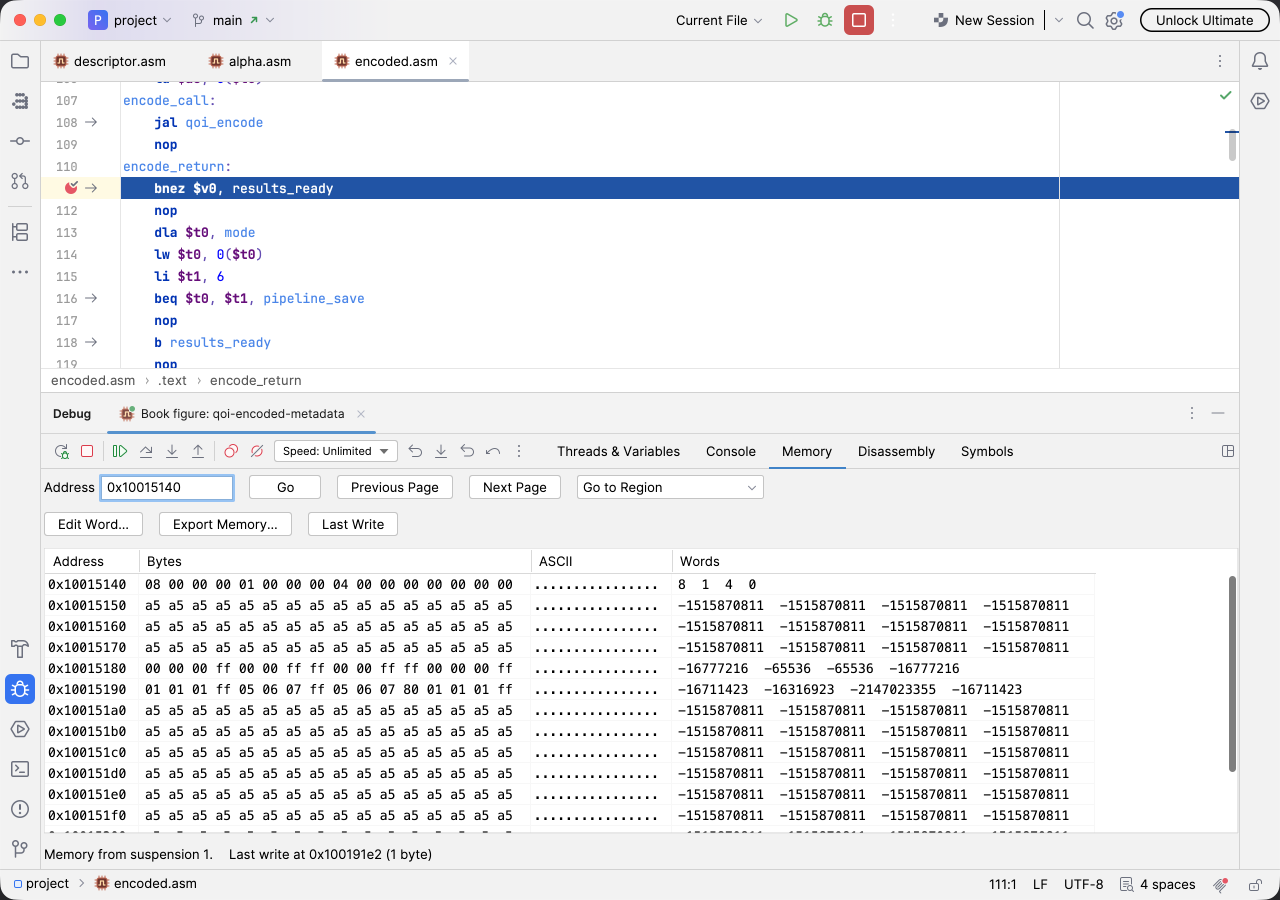
\includegraphics[width=0.84\linewidth,artifact,trim={\MARSqoiencodedmetadataLeft{} \MARSqoiencodedmetadataBottom{} \MARSqoiencodedmetadataRight{} \MARSqoiencodedmetadataTop{}},clip]{packages/030-qoi/captures/f03/metadata.png}};
    \begin{scope}[shift={(metadata.south west)},x={($(metadata.south east)-(metadata.south west)$)},y={($(metadata.north west)-(metadata.south west)$)}]
      \draw[black,line width=0.7pt] (0.194672131,0.078431373) rectangle (0.997950820,0.490196078);
      \node[draw=black,fill=white,circle,inner sep=1.5pt,font=\footnotesize] at ($(0,0.490196078)+(-3mm,0)$) {5};
    \end{scope}
  \end{tikzpicture}
  \par\smallskip
  \begin{minipage}{\linewidth}
    \small
    \begin{enumerate}
      \setlength{\itemsep}{0pt}
            \setlength{\parsep}{0pt}
      \item At \texttt{encode\_return}, the encoder has finished and restored its frame. The caller has not yet copied the return values into its saved controls.
      \item \texttt{v0 = 0} reports success, and \texttt{v1 = 35} is the complete output length. Unlike the validator\textquotesingle s pixel count or decoder\textquotesingle s packed dimensions, this interface returns bytes.
      \item The output has the same fourteen-byte header and eight-byte marker as the worked source. After its initial \texttt{c0} run, \texttt{5a} encodes the change from black to red using a wrapped red difference of $-1$ and zero green and blue differences. It replaces the original four-byte \texttt{fe ff 00 00} command, saving three bytes. Output ends after thirty-five bytes; the following \texttt{a5} suffix is untouched.
      \item The original framebuffer words remain unchanged, including both alpha values near its end. Compression chooses chunk representations; it does not discard alpha or approximate the colors. An independent reference decoder recovers all eight original RGBA values from this stream.
      \item The input metadata still contains width eight, height one, channels four and colorspace zero. Both descriptive flags survive in the header. Equivalent valid encoders may choose different chunks; complete grading checks the recovered image and stated bounds rather than requiring this exact byte sequence.
    \end{enumerate}
  \end{minipage}
  \caption{The encoder returns a shorter stream that preserves every pixel and both flags.}
  \label{capture:030-qoi-f03}
  \label{qoi-f03}
\end{figure}
\par
